\addcontentsline{toc}{chapter}{Занятие 17. Центральная предельная теорема}
\chapter*{Занятие 17. Центральная предельная теорема}

\addcontentsline{toc}{section}{Контрольные вопросы и задания}
\section*{Контрольные вопросы и задания}

\subsubsection*{Сформулируйте центральную предельную теорему,
                запишите центральную предельную теорему для последовательности испытаний Бернулли.}

Центральная предельная теорема.
$ \xi_1, \dotsc, \xi_n$ -- независимые одинаково распределённые случайные величины,
$M \xi_1 = a, \,
  D \xi_1 = \sigma^2 < \infty $.
Тогда
$$ \frac{S_n - MS_n}{ \sqrt{D \xi_1}} \overset{d}{ \rightarrow } N \left( 0, 1 \right), \,
  n \to \infty,$$
где
$$S_n =
  \sum \limits_{i = 1}^n \xi_i.$$

Подставляя значения математического ожидания и дисперсии получим
$$ \frac{S_n - na}{ \sqrt{n}} \overset{d}{ \rightarrow } N \left( 0, \sigma^2 \right), \
  n \to \infty.$$

Пусть $ \left\{ \varepsilon_k \right\} $ ---
последовательность независимых одинаково распределённых случайных величин, таких, что
$$ \varepsilon_k =
  \begin{cases}
    1, \qquad p, \\
    0, \qquad 1 - p.
  \end{cases}$$
Тогда
$$ \frac{S_n - np}{ \sqrt{n}} \overset{d}{ \rightarrow }
  N \left( 0, p \left( 1 - p \right) \right).$$

Перенесём $p \left( 1 - p \right)$ влево
$$ \frac{S_n - np}{ \sqrt{n} \sqrt{p \left( 1 - p \right) }} \overset{d}{ \rightarrow }
  N \left( 0, 1 \right).$$

\addcontentsline{toc}{section}{Аудиторные задачи}
\section*{Аудиторные задачи}

\subsubsection*{17.3}

\textit{Задание.} Пусть $ \xi $ --- случайная величина со стандартным нормальным распределением.
Пользуясь таблицей стандартного нормального распределения найдите:
\begin{enumerate}[label=\alph*)]
\item вероятность $P \left( \xi \leq 2.2 \right) $;
\item такое $x$, что $P \left( \xi > x \right) = 0.9$.
\end{enumerate}

\textit{Решение.} $ \xi \sim N \left( 0 ,1 \right) $.
Найдём вероятности
\begin{enumerate}[label=\alph*)]
\item $P \left( \xi \leq 2.2 \right) =
        1 -P \left( \xi > 2.2 \right) =
        1 - \Phi_t \left( 2.2 \right) =
        1 - 0.014 =
        -.986$;
\item изобразим ситуацию на рисунке \ref{fig:173}.

\begin{figure}[h!]
  \centering
  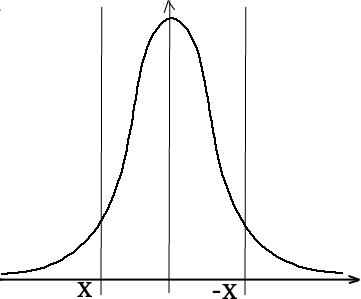
\includegraphics[width=.4\textwidth]{./pictures/17_3.png}
  \caption{Площадь под гауссианой}
  \label{fig:173}
\end{figure}

Площадь каждой половины под графиком равна $0.5$.
Отсюда следует, что $x < 0$.

Получаем, что $ \Phi_t \left( -x \right) = 0.1$.

Ещём в таблице значений $-x = 1.18$.
Значит, $x = -1.18$.
\end{enumerate}

\subsubsection*{17.4}

\textit{Задание.}
Пусть $S_{100}$ --- число гербов, которые выпали при 100 подбрасываниях правильной монеты.
С помощью центральной предельной теоремы приближённо вычислите вероятности:
$$P \left( S_{100} < 45 \right), \,
  P \left( 45 < S_{100} < 55 \right), \,
  P \left( S_{100} > 63 \right).$$

\textit{Решение.} Пусть $ \xi_i = \mathbbm{1}$ \{при $i$-м подбрасывании выпал герб\}.
Тогда
$$S_{100} =
  \sum \limits_{i = 1}^{100} \xi_i.$$

Математическое ожидание введённой случайной величины совпадает с вероятностью того, что выпал герб
$$M \xi_i =
 \frac{1}{2}.$$

Дисперсия равна
$$D \xi_i =
  \frac{1}{2} \cdot \frac{1}{2} =
  \frac{1}{4}.$$

Для суммы
$$MS_{100} = 100 \cdot \frac{1}{2} = 50, \,
  DS_{100} = \frac{100}{4} = 25.$$

Найдём первую вероятность
$$P \left( S_{100} < 45 \right) =
  P \left(
      \frac{S_{100} - MS_{100}}{ \sqrt{DS_{100}}} < \frac{45 - MS_{100}}{ \sqrt{DS_{100}}}
    \right).$$
Первая дробь в скобрах примерно равна случайной величине
$$ \eta \to
  N \left( 0, 1 \right)$$
по центральной предельной теореме
$$P \left( S_{100} < 45 \right) =
  P \left( \eta < \frac{45 - 50}{ \sqrt{25}} \right) =
  P \left( \eta < -1 \right) =
  P \left( \eta > 1 \right) =
  0.159.$$

Следующая вероятность равна
$$P \left( 45 < S_{100} < 55 \right) =
  P \left( -1 < \eta < 1 \right) =
  1 - 2 \Phi_t \left( 1 \right) =
  1 - 2 \cdot 0.159 =
  0.682.$$

Последняя верноятность из таблицы равна
$$P \left( S_{100} > 63 \right) =
  P \left( \eta > \frac{13}{5} \right) =
  P \left( \eta > 2.6 \right) =
  0.005.$$

\subsubsection*{17.5}

\textit{Задание.}
Пусть $ \left\{ \xi_n \right\}_{n \geq 1}$ ---
последовательность независимых одинаково распределённых
случайных величин с распределением Бернулли с параметром
$$p =
  \frac{1}{2},$$
и пусть $S_k = \xi_1 + \dotsc + \xi_k$.
Найдите такое $k$, чтобы
$$P \left( \left| S_k - kp \right| > 1000 \right) >
  0.0455.$$

\textit{Решение.} Математическое ожидание суммы $S_k$ равно
$$MS_K =
  kp =
  k \cdot \frac{1}{2}.$$

Дисперсия равна
$$DS_k =
  k \cdot \frac{1}{4}.$$

Записываем вероятность в таком виде, чтобы можно было применить центральную предельную теорему
$$P \left( \left| S_k - \frac{k}{2} \right| > 1000 \right) =
  P \left(
      \left| \frac{S_k - \frac{k}{2}}{ \sqrt{ \frac{k}{4}}} \right| > \frac{2000}{ \sqrt{k}}
    \right) \approx
  P \left( \left| \eta \right| > \frac{2000}{ \sqrt{k}} \right) >
  0.0455,$$
так как
$$ \frac{S_k - \frac{k}{2}}{ \sqrt{ \frac{k}{4}}} \approx
  \eta \sim
  N \left( 0, 1 \right).$$

Нарисуем график (рис. \ref{fig:175}), закрасим площадь, котороя соответствует тому, что
$$ \left| \eta \right| >
  \frac{1000}{ \sqrt{k}} =
  x.$$

\begin{figure}[h!]
  \centering
  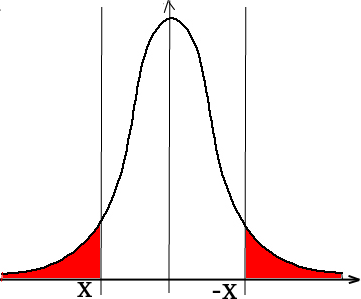
\includegraphics[width=.4\textwidth]{./pictures/17_5.png}
  \caption{Площадь под гауссианой}
  \label{fig:175}
\end{figure}

Тогда
$$2 \Phi_t \left( \frac{2000}{ \sqrt{k}} \right) >
  0.0455.$$

Тогда табличное
$$ \Phi_t \left( \frac{2000}{ \sqrt{k}} \right) >
  0.0275.$$

В таблице значений ищем $0.0275 \approx 0.028$.
Получается
$$ \frac{2000}{ \sqrt{k}} <
  1.91.$$

Отсюда
$$ \sqrt{k} >
  \frac{2000}{1.91} \approx
  \frac{2000}{2} =
  1000.$$
Тогда $k > 10000000$.

\subsubsection*{17.6}

\textit{Задание.}
Найдите вероятность того, что в случайном наборе из 10 000 цифр цифра 3 появится не больше 931 раза.

\textit{Решение.} Есть $10000 = N$ испытаний.

$ \xi_i = \mathbbm{1} \left\{ A_i \right\},$
где $A_i =$ \{в $i$-м испытании появилась тройка\}.
$$M \xi_i =
  P \left( A_i \right) =
  \frac{1}{10}.$$

Дисперсия введённой случайной величины равна
$$D \xi_i =
  \frac{1}{10} \cdot \frac{9}{10} =
  \frac{9}{100}.$$

Введём
$$S_{10000} =
  \sum \limits_{i = 1}^{10000} \xi_i.$$
Тогда математическое ожидание такое суммы равно
$$MS_{10000} =
  10000 \cdot \frac{1}{10} =
  1000,$$
а дисперсия $DS_{10000} = 900$.
Таким образом,
$$P \left( S_{10000} \leq 931 \right) =
  P \left(
    \frac{S_{10000} - MS_{10000}}{ \sqrt{DS_{10000}}} \leq \frac{931 - MS_{10000}}{ \sqrt{DS_{10000}}}
  \right).$$
Подставим значения математического ожидания и дисперсии
$$P \left( S_{10000} \leq 931 \right) =
  P \left( \frac{S_{10000} - 1000}{30} \leq \frac{931 - 1000}{30} \right).$$
Упростим выражение справа
$$P \left( S_{10000} \leq 931 \right) =
  P \left( \frac{S_{10000} - 1000}{30} \leq -\frac{23}{10} \right) =
  \Phi_t \left( 2.3 \right) =
  0.011.$$

\subsubsection*{17.8}

\textit{Задание.} В некоторой группе людей дальтоники составляют в среднем 1\% людей.
Насколько большой должна быть выборка,
чтобы вероятность наличия в ней хотя бы одного дальтоника была не меньшей чем $0.95$?

\textit{Решение.} $n$ --- размер выборки.

$ \xi_i = \mathbbm{1}$ \{$i$-тый человек является дальтоником\}.

Тогда количество дальтоников в выборке из $n$ людей
$$S_n =
  \sum \limits_{i = 1}^n \xi_i.$$

Математическое ожидание равно
$$MS_n =
  \frac{n}{100},$$
потому что
$$M \xi_i =
  \frac{1}{100}.$$

Дисперсия случайной величины равна
$$D \xi_i =
  \frac{1}{100} \cdot \frac{99}{100} =
  \frac{99}{10000} \approx
  \frac{1}{100}.$$

Тогда
$$DS_n \approx
  \frac{n}{100}.$$

Нужно, чтобы выполнялось $P \left( S_n \geq 1 \right) \geq 0.95$.
Из этого условия найдём $n$.

Преобразовываем событие в вероятности так, чтобы применить центральную предельную теорему
$$P \left( S_n \geq 1 \right) =
  P \left\{
    \left( S_n - \frac{n}{100} \right) \cdot \frac{ \sqrt{100}}{\sqrt{n}} \geq
    \frac{1 - \frac{n}{100}}{ \sqrt{ \frac{n}{100}}}
  \right\}.$$
То, что стоит до знака <<не меньше>>, примерное равно случайной величине
$ \eta \to N \left( 0, 1 \right) $.
Обозначим правую часть неравенства через $x$.

Таблично это будет выглядеть так $ \Phi_t \left( -x \right) < 0.05$.

В таблице ищем значение.
Это будет $-x > 1.65, \, x < -1.65$.

Нужно теперь решить квадратное уравнение
$$ \frac{1 - \frac{n}{100}}{ \sqrt{ \frac{n}{100}}} < -1.65.$$

Сделаем замену $ \sqrt{n} = t$ и умножим обе части неравенства на знаменатель и на $-100$,
а также перенесём всё влево.
Получим $t^2 - 16.5t - 100 > 0$.
Дискриминант соответствующего уравения равен
$$D =
  \left( 16.5 \right)^2 + 4 \cdot 100 =
  272.25 + 400 =
  672.25 \approx
  \left( 25.93 \right)^2.$$
Находим корень (отрицательный не подходит)
$$t =
  \frac{16.5 + 25.93}{2} =
  21.215.$$
Возвращаемся к замене $ \sqrt{n} > 21.215$, откуда $n >  \left( 21.215 \right)^2 \approx 450$.

\subsubsection{17.9}

\textit{Задание.} Некоторое село насчитывает 2500 жителей.
Каждый из них в среднем 6 раз в меесяц ездит на электричке в город,
выбирая дни поездок по случайным причинам и независимо от других жителей.
Какую наименьшую ёмкость должна иметь электричка,
чтобы она переполнялась в среднем не чаще одного раза за сто дней
(электричка курсирует раз в сутки).

\textit{Решение.} В месяце 30 дней.
Введём случайную величину $ \xi_i = \mathbbm{1}$ \{$i$-й человек в определённый день месяца едет в город\}.

По условию задачи
$$M \xi_i =
  \frac{6}{30} =
  \frac{1}{5}$$
--- это вероятность того, что человек едет в город.

Тогда дисперсия
$$D \xi_i =
  pq =
  \frac{1}{5} \cdot \frac{4}{5} =
  \frac{4}{25},$$
где $p$ --- вероятность того, что человек едет в город, $q = 1 - p$ --- вероятность того,
что человек не едет в город.

$S_{2500} = \xi_1 + \dotsc + \xi_{2500}$ --- количество занятых мест в электричке.

$$MS_{2500} =
  \frac{2500}{5} =
  500,$$
в среднем будет ездить 500 людей в день, а дисперсия
$$DS_{2500} =
  \frac{2500 \cdot 4}{25} =
  400.$$

То, что случилось переполнение, означает, что $S_{2500} \geq x$, где $x$ ---
количество мест в электричке.

$$P \left\{ S_{2500} \geq x \right\} <
  \frac{1}{100}.$$

Согласно с центральной предельной теоремой,
$$ \frac{S_{2500} - MS_{2500}}{ \sqrt{DS_{2500}}} =
  \eta \sim
  N \left( 0, 1 \right).$$

В неравенстве под знаком вероятности делаем так, чтобы там возникла $ \eta $.
Подставляем значения
$$P \left\{ \eta \geq \frac{x - 500}{20} \right\} <
  \frac{1}{100}.$$

Рисуем график плотности нормального закона (рис. \ref{fig:179}).

\begin{figure}[h!]
  \centering
  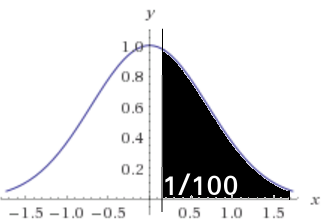
\includegraphics[width=.4\textwidth]{./pictures/17_9.png}
  \caption{Площадь под гауссианой}
  \label{fig:179}
\end{figure}

Это табличное значение
$$ \Phi_t \left( \frac{x - 500}{20} \right) <
  \frac{1}{100} =
  0.01.$$

Из таблицы нормального распределения находим, что
$$ \frac{x - 500}{20} >
  2.33.$$

Умножим правую и левую части на знаменатель $x - 500 > 46.6$.

Отсюда $x > 546.6.$

Наименьшее $x = 547$.

\subsubsection{17.10}

\textit{Задание.} Ресторан обслуживает 400 посетителей ежедневно.
В среднем 20\% посетителей заказывают на десерт кусок яблочного пирога.
Укажите границы,
в которых с вероятностью не меньшей чем $0.95$
лежит количество заказанных за день кусков яблочного пирога.
Сколько посетителей в среднем должен ежедневно обслуживать ресторан,
чтобы с вероятностью $0.95$ количество заказанных кусков яблочного пирога была не меньшей чем 20?

\textit{Решение.} $ \xi_i = \mathbbm{1}$ \{$i$-й человек заказал яблочный пирог\}.

Тогда количество кусков пирока, которые заказали за день --- это будет
$$S_{400} =
  \sum \limits_{i = 1}^{400} \xi_i.$$

Количество пирогов колеблется относительно своего среднего
$$M \xi_i = \frac{1}{5}, \,
  MS_{400} = \frac{400}{5} = 80,$$
соответственно
$$D \xi_i = \frac{4}{25}, \,
DS_{400} = \frac{400 \cdot 4}{25} = 64.$$

Нужно оценить $x_1$ и $x_2$ в вероятности $P \left( x_1 < S_{400} < x_2 \right) \geq 0.95$.

Оценить сразу 2 параметра мы не можем.

Будем искать у виде $S_{400} = 80 \pm x$.
Этот $x$ и будем искать.


$P \left( \left| S_{400} - 80 \right| < x \right) \geq 0.95$.

Свели задачу к задаче с одним параметром.

Чтобы применить центральную предельную теорему, нужно поделить на корень из дисперсии
$$P \left( \frac{S_{400} - 80}{8} < \frac{x}{8} \right) \geq
  0.95.$$

Это будет площадь под гауссианой между $- x / 8$ и $x / 8$.
Из неравенства
$$1 - 2 \Phi_t \left( \frac{x}{8} \right) \geq
  0.95$$
ищем неравенство для функции
$$ \Phi_t \left( \frac{x}{8} \right) \leq
  0.025.$$

В таблице находим
$$ \frac{x}{8} \geq
  1.96 \approx
  2.$$

Значит, $x > 16$.

Количество пирогов должно быть от 64 до 96.

\addcontentsline{toc}{section}{Домашнее задание}
\section*{Домашнее задание}

\subsubsection*{17.11}

\textit{Задание.} Пусть $ \xi $ --- случайная величина со стандартным нормальным распределением.
Пользуясь таблицей стандартного нормального распределения найдите:
\begin{enumerate}[label=\alph*)]
\item вероятность $P \left( \xi \in \left[ -3, 1 \right] \right) $;
\item такое $x$, что $P \left( \left| \xi \right| \leq x \right) = 0.9$.
\end{enumerate}

\textit{Решение.}
\begin{enumerate}[label=\alph*)]
\item Разобъём искомую вероятность на разность двух
$$P \left( \xi \in \left[ -3, 1 \right] \right) =
  P \left( \xi \geq -3 \right) - P \left( \xi > 1 \right) =
  \Phi_t \left( -3 \right) - \Phi_t \left( 1 \right).$$
Преобразуем первое слагаемое, чтобы был положительный аргумент
$$P \left( \xi \in \left[ -3, 1 \right] \right) =
  1 - \Phi_t \left( 3 \right) - \Phi_t \left( 1 \right) =
  1 - 0.00135 - 0.0159 =
  0.83965;$$
\item из условия находим, что $1 - 2 \Phi_t \left( x \right) = 0.9$.
Отсюда
$$2 \Phi_t \left( x \right) =
  1 - 0.9 =
  0.1.$$
Делим на $2$ и получаем $ \Phi_t \left( x \right) = 0.05$.
В таблице находим, что
$$x =
  1.645.$$
\end{enumerate}

\subsubsection*{17.12}

\textit{Задание.}
Пусть $S$ --- число гербов, что выпали при 1 000 000 подбрасываниях правильной монеты.
Оцените вероятность $P \left( 499000 < S < 501000 \right) $:
\begin{enumerate}[label=\alph*)]
\item с помощью неравенства Чебышева;
\item с помощью центральной предельной теоремы.
\end{enumerate}

\textit{Решение.} Пусть $ \xi_i = \mathbbm{1}$ \{при $i$-м подбрасывании выпал герб\}.
Тогда
$$S =
  \sum \limits_{i = 1}^{1000000} \xi_i.$$

Математическое ожидание введённой случайной величины совпадает с вероятностью того, что выпал герб
$$M \xi_i =
  \frac{1}{2}.$$

Дисперсия равна
$$D \xi_i =
  \frac{1}{2} \cdot \frac{1}{2} =
  \frac{1}{4}.$$

Для суммы
$$MS = 1000000 \cdot \frac{1}{2} = 500000, \,
  DS = \frac{1000000}{4} = 250000.$$

\begin{enumerate}[label=\alph*)]
\item Воспользуемся неравенством Чебышева для дисперсии
$$P \left( \left| \xi - M \xi \right| \geq \varepsilon \right) \leq
  \frac{D \xi }{ \varepsilon^2}$$
или
$$P \left( \left| \xi - M \xi \right| < \varepsilon \right) \geq
  1 - \frac{D \xi }{ \varepsilon^2}.$$

Отнимем от всех частей неравенства математическое ожидание суммы
\begin{equation*}
  \begin{split}
    P \left( 499000 < S < 501000 \right) =
    P \left( 499000 - MS < S - MS < 501000 - MS \right) = \\
    = P \left( 499000 - 500000< S - MS < 501000 - 500000 \right) = \\
    = P \left( -1000 < S - MS < 1000 \right) =
    P \left( \left| S - MS \right| < 1000 \right) \geq \\
    \geq 1 - \frac{DS}{1000^2} =
    1 - \frac{250000}{1000000} =
    1 - 0.25 =
    0.75;
  \end{split}
\end{equation*}
\item в предыдущем пункте получили,
что
$$P \left( 499000 < S < 501000 \right) =
  P \left( \left| S - MS \right| < 1000 \right).$$
Поделим правую и левую части на корень из дисперсии суммы
$$P \left( 499000 < S < 501000 \right) =
  P \left( \frac{ \left| S - MS \right| }{ \sqrt{DS}} < \frac{1000}{ \sqrt{DS}} \right).$$
В правой части подставим значение дисперсии
$$P \left( 499000 < S < 501000 \right) =
  P \left( \frac{ \left| S - MS \right| }{ \sqrt{DS}} < \frac{1000}{500} \right).$$
Поделим в правой части константы
$$P \left( 499000 < S < 501000 \right) =
  P \left( \frac{ \left| S - MS \right| }{ \sqrt{DS}} < 2 \right) =
  1 - 2 \Phi_t \left( 2 \right).$$
Найдём в таблице нормального распределения соответствующее значение
$$P \left( 499000 < S < 501000 \right) =
  1 - 2 \cdot 0.023 =
  1 - 0.046 =
  0.954.$$
\end{enumerate}

\subsubsection*{17.13}

\textit{Задание.}
Пусть $ \xi_1, \xi_2, \dotsc $ ---
последовательность независимых случайных величин с распределением Бернулли с параметром
$$p =
  \frac{1}{2},$$
и пусть $S_k = \xi_1 + \dotsc + \xi_k$.
Найдите такое $k$, что $P \left( \left| S_k - kp \right| > 100 \right) < 0.05$.

\textit{Решение.} Математическое ожидание суммы $S_k$ равно
$$MS_k =
  kp =
  k \cdot \frac{1}{2}.$$

Дисперсия равна
$$DS_k =
  k \cdot \frac{1}{4}.$$

Запишем вероятность в таком виде, чтобы можно было применить центральную предельную теорему
$$P \left( \left| S_k - \frac{k}{2} \right| > 100 \right) =
  P \left(
    \left| \frac{S_k - \frac{k}{2}}{ \sqrt{ \frac{k}{4}}} \right| > \frac{100}{ \sqrt{ \frac{k}{4}}}
  \right) \approx
  P \left( \left| \eta \right| > \frac{200}{ \sqrt{k}} \right) <
  0.05,$$
так как
$$ \frac{S_k - \frac{k}{2}}{ \sqrt{ \frac{k}{4}}} \approx
  \eta \sim
  N \left( 0, 1 \right).$$

Соответствующий график изображён на рисунке \ref{fig:175}, закрашена площадь,
которая соответствует тому, что
$$ \left| \eta \right| >
  \frac{200}{ \sqrt{k}} =
  x.$$

Тогда
$$2 \Phi_t \left( \frac{200}{ \sqrt{k}} \right) < 0.05.$$

Выражаем табличное значение
$$ \Phi_t \left( \frac{200}{ \sqrt{k}} \right) <
  \frac{0.05}{2} =
  0.025.$$

В таблице значений ищем $0.025$.
Это соответствует тому, что
$$ \frac{200}{ \sqrt{k}} >
  1.96.$$

Отсюда
$$ \sqrt{k} <
  \frac{200}{1.96} \approx
  102.04.$$
Подносим в квадрат и получаем $k < 10412.16$.

\subsubsection*{17.14}

\textit{Задание.}
При случайном блуждании на числовой оси частица, стартуя из точки 0,
делает шаг вправо или влево с вероятностями $1 / 2$.
Оцените вероятность того, что после сотого шага частицу будет отдалять от начальной точки не меньше,
чем 10 шагов.

\textit{Решение.} Введём случайную величину, соответствующую перемешению вправо или влево
$$ \xi_i =
  \begin{cases}
    1, \qquad \frac{1}{2}, \\
    -1, \qquad \frac{1}{2}.
  \end{cases}$$
Тогда количество шагов, которые будут отдалять частицу от начальной точки после сотого шага равно
$$S_{100} =
  \sum \limits_{i = 1}^{100} \xi_i.$$

Математическое ожидание введённой случайной величины по определению равно
$$M \xi_i =
  1 \cdot \frac{1}{2} - 1 \cdot \frac{1}{2} =
  0.$$

Дисперсия совпадает со вторым моментом
$$D \xi_i =
  M \xi_i^2 =
  1^2 \cdot \frac{1}{2} + \left( -1 \right)^2 \cdot \frac{1}{2} =
  \frac{1}{2} + \frac{1}{2} =
  1.$$

Для суммы $MS_{100} = 100 \cdot 0 = 0, \, DS_{100} = 100 \cdot 1 = 100$.

Найдём вероятность
$$P \left( \left| S_{100} \right| \geq 10 \right) =
  P \left(
    \frac{ \left| S_{100} \right| - MS_{100}}{ \sqrt{DS_{100}}} \geq
    \frac{10 - MS_{100}}{ \sqrt{DS_{100}}}
  \right).$$

Первая дробь стремится к случайной величине $ \eta \sim N \left( 0, 1 \right) $
по центральной предельной теореме.
$$P \left( \left| S_{100} \right| \geq 10 \right) =
  P \left( \eta \geq \frac{10 - 0}{ \sqrt{100}} \right) =
  P \left( \eta \geq \frac{10}{10} \right) =
  P \left( \eta \geq 1 \right) =
  \Phi_t \left( 1 \right).$$
В таблице нормального распределения находим значение для единицы
$$P \left( \left| S_{100} \right| \geq 10 \right) =
  0.159.$$
